% From report/epistemics/figures, run xelatex experiment-architecture.tex.
% Architecture source: harness/research/sector-expansion/ARCHITECTURE.md.
% Palette and typography: website/src/styles/global.css.
\documentclass[tikz,border=0pt]{standalone}
\usepackage{fontspec}
\IfFontExistsTF{Iowan Old Style}
  {\setmainfont{Iowan Old Style}}
  {\setmainfont{TeX Gyre Pagella}}
\usetikzlibrary{arrows.meta}

\definecolor{paper}{HTML}{FAFAF9}
\definecolor{cream}{HTML}{EEE9DC}
\definecolor{ivory}{HTML}{FAF7ED}
\definecolor{forest}{HTML}{193E32}
\definecolor{leaf}{HTML}{24523F}
\definecolor{muted}{HTML}{62665B}
\definecolor{stone}{HTML}{D6D3D1}

\begin{document}
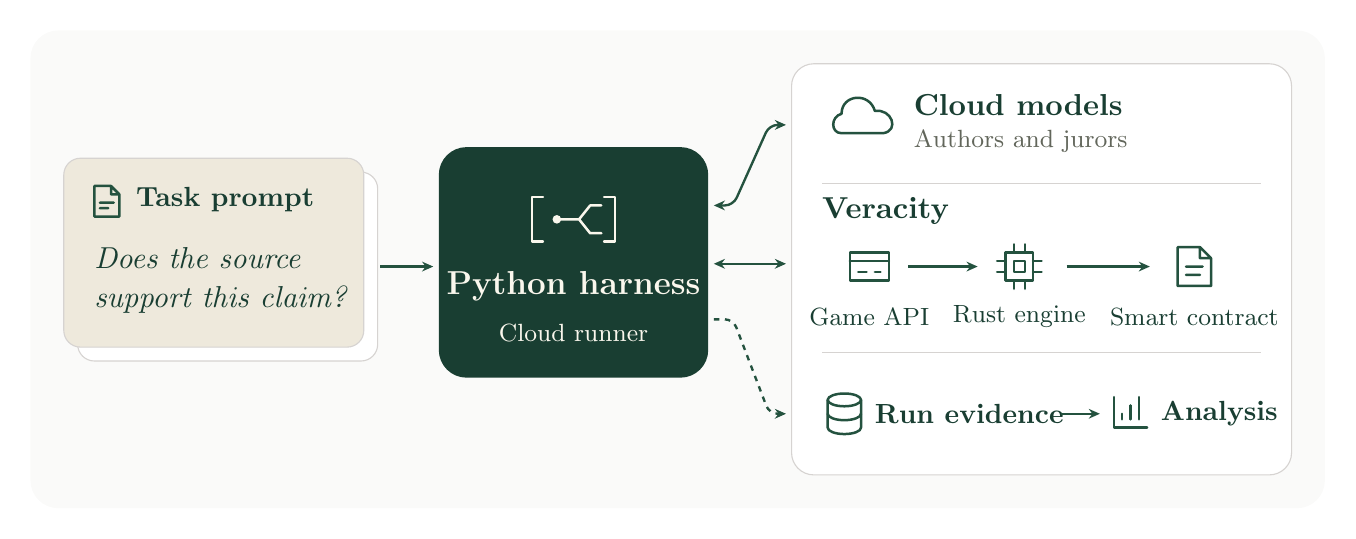
\begin{tikzpicture}[
  x=1bp, y=1bp,
  every node/.style={inner sep=0pt, outer sep=0pt, text=forest},
  heading/.style={font=\fontsize{11}{13}\selectfont\bfseries},
  detail/.style={font=\fontsize{9}{11}\selectfont},
  icon/.style={draw=leaf, line width=.9bp, line join=round, line cap=round},
  flow/.style={draw=leaf, line width=.85bp, -{Stealth[length=4bp,width=3.5bp]}},
  exchange/.style={flow, {Stealth[length=4bp,width=3.5bp]}-{Stealth[length=4bp,width=3.5bp]}},
  evidence/.style={flow, dash pattern=on 2bp off 2bp},
]
\path[use as bounding box] (0,0) rectangle (468,174);
\fill[paper,rounded corners=10bp] (1,1) rectangle (467,173);

% On the left, the visible text is an example of the prompt a model receives.
\draw[stone,fill=white,rounded corners=6bp] (18,54) rectangle (126,122);
\draw[stone,fill=cream,rounded corners=6bp] (13,59) rectangle (121,127);
\draw[icon] (24,117) -- (30,117) -- (33,114) -- (33,106) -- (24,106) -- cycle
  (30,117) -- (30,114) -- (33,114) (26,111) -- (31,111) (26,109) -- (29,109);
\node[heading,anchor=west,font=\fontsize{10}{12}\selectfont\bfseries]
  at (39,112) {Task prompt};
\node[anchor=west,align=left,font=\fontsize{11}{14}\selectfont\itshape]
  at (24,83) {Does the source\\support this claim?};
\draw[flow] (127,88) -- (146,88);

% The harness is the focal point. Its three paths have distinct destinations.
\fill[forest,rounded corners=10bp] (148,48) rectangle (245,131);
\begin{scope}[icon,draw=ivory,shift={(196.5,105)}]
  \draw (-11,8) -- (-15,8) -- (-15,-8) -- (-11,-8)
    (11,8) -- (15,8) -- (15,-8) -- (11,-8);
  \draw (-5,0) -- (2,0) -- (6,5) -- (10,5)
    (2,0) -- (6,-5) -- (10,-5);
  \fill[ivory,draw=none] (-6,0) circle (1.55bp);
\end{scope}
\node[text=ivory,font=\fontsize{11.6}{14}\selectfont\bfseries]
  at (196.5,81) {Python harness};
\node[text=ivory,detail] at (196.5,64) {Cloud runner};

% The bands on the right trace inference, dispute execution and evidence.
\draw[stone,fill=white,rounded corners=8bp] (275,13) rectangle (455,161);
\draw[stone,line width=.5bp] (286,118) -- (444,118) (286,57) -- (444,57);
\draw[exchange,rounded corners=3bp] (247,110) -- (254,110) -- (267,139) -- (273,139);
\draw[exchange] (247,89) -- (273,89);
\draw[evidence,rounded corners=3bp] (247,69) -- (254,69) -- (267,35) -- (273,35);

\draw[icon,shift={(290,136)}]
  (3,0) .. controls (-1,0) and (-1,6) .. (3,7)
  .. controls (3,14) and (13,15) .. (15,8)
  .. controls (21,9) and (24,1) .. (18,0) -- cycle;
\node[heading,anchor=west] at (319,146) {Cloud models};
\node[detail,anchor=west,text=muted] at (319,133) {Authors and jurors};

\node[heading,anchor=west] at (286,108) {Veracity};
\begin{scope}[icon,shift={(303,88)}]
  \draw (-7,-5) rectangle (7,5);
  \draw (-7,2) -- (7,2) (-4,-2) -- (-1,-2) (2,-2) -- (4,-2);
\end{scope}
\begin{scope}[icon,shift={(357,88)}]
  \draw (-5,-5) rectangle (5,5);
  \draw (-2,-2) rectangle (2,2);
  \draw (-2,5) -- (-2,8) (2,5) -- (2,8) (-2,-5) -- (-2,-8) (2,-5) -- (2,-8)
    (-5,-2) -- (-8,-2) (-5,2) -- (-8,2) (5,-2) -- (8,-2) (5,2) -- (8,2);
\end{scope}
\begin{scope}[icon,shift={(420,88)}]
  \draw (-6,-7) -- (6,-7) -- (6,3) -- (2,7) -- (-6,7) -- cycle
    (2,7) -- (2,3) -- (6,3) (-3,0) -- (3,0) (-3,-3) -- (2,-3);
\end{scope}
\draw[flow] (317,88) -- (342,88);
\draw[flow] (374,88) -- (404,88);
\node[detail] at (303,70) {Game API};
\node[detail] at (357,70) {Rust engine};
\node[detail] at (420,70) {Smart contract};

\begin{scope}[icon,shift={(294,34)}]
  \draw (0,6) ellipse (6bp and 2.3bp);
  \draw (-6,6) -- (-6,-4) arc[start angle=180,end angle=360,x radius=6bp,y radius=2.3bp] -- (6,6);
  \draw (-6,1) arc[start angle=180,end angle=360,x radius=6bp,y radius=2.3bp];
\end{scope}
\node[anchor=west,font=\fontsize{10}{12}\selectfont\bfseries]
  at (305,35) {Run evidence};
\draw[flow] (372,35) -- (386,35);
\begin{scope}[icon,shift={(397,35)}]
  \draw (-6,6) -- (-6,-5) -- (6,-5);
  \draw (-3,-2) -- (-3,0) (0,-2) -- (0,3) (3,-2) -- (3,6);
\end{scope}
\node[anchor=west,font=\fontsize{10}{12}\selectfont\bfseries]
  at (408,35) {Analysis};
\end{tikzpicture}
\end{document}
